% This is LLNCS.DEM the demonstration file of
% the LaTeX macro package from Springer-Verlag
% for Lecture Notes in Computer Science,
% version 2.2 for LaTeX2e
%
\documentclass[runningheads]{llncs}
\usepackage{makeidx}  % allows for indexgeneration
\usepackage{graphicx} %includegraphics
\usepackage{multirow}
\usepackage{rotating}
\usepackage{subfigure}
\usepackage{array}
\usepackage{hyperref}


%
\begin{document}
%
%% \frontmatter          % for the preliminaries
%
\pagestyle{headings}  % switches on printing of running heads
%
\title{Parallelization of 2-d Ising Model}
\titlerunning{Parallilization of 2-d Ising model}

\author{Sean Rivera, Michael Winterfeld, Kenneth Sheedlo, Honghua Yang$^{\dagger}$}
%\email{honghua.yang@colorado.edu}
\authorrunning{Rivera et al.}

\institute{honghua.yang@colorado.edu \\
University of Colorado, Boulder, CO }


\maketitle              % typeset the title of the contribution

\begin{abstract}
The Ising model, named after the physicist Ernst Ising, is a mathematical model of ferromagnetism in statistical mechanics. The model allows the identification of phase transitions, as a simplified model of more complicated reality. In this project we will study this model by Monte Carlo simulation implemented in C and MPI, in addition we will compare the performance of serial code and parallel code by speedup.

\end{abstract}

\section{Introduction}
Ising model consists of discrete values that represent magnetic dipole moments of atomic spins that can be in one of two states (+1 or −1). The spins are arranged in a lattice allowing each spin to interact with its neighbors.
Depending on the interaction, the spin system undergoes a phase transition at different temperature.


\section{Description of the Problem}
We will consider interacting spins on a 2-d square lattice with Hamiltonian:
\begin{equation}
\mathcal{H} = -\sum_{\left<ij\right>}s_is_j 
\end{equation}
where the notation  $\left<ij\right>$ denotes that we are summing over unique pairs of nearest neighbors.

The goal of this project is to parallelize the Metropolis simulation of 2-d Ising model, and compare the performance of the serial code and the parallel code using strong scaling and weak scaling.

The input data of the problem is the temperature  with randomly initialized 2-d of spins. 
The output would be the energy of the thermalized system and the average magnetization.
We will also try to implement a graphic window to display the evolution of the system.
\begin{figure}
\begin{center}
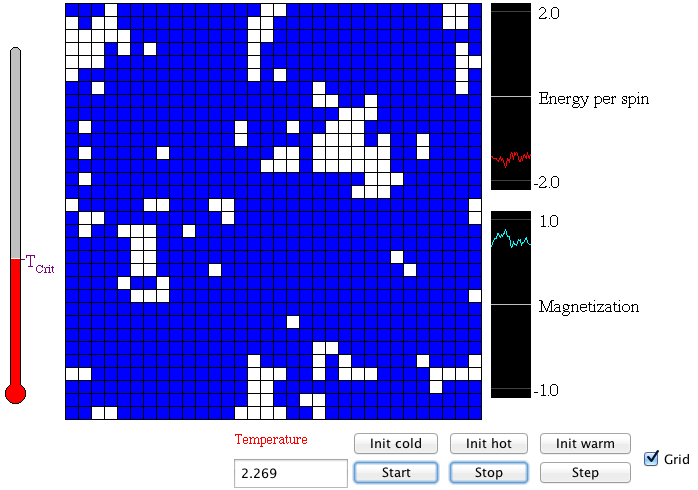
\includegraphics[width=3.5in]{./Ising_graphic.png}
\caption[]{ Illustration of a Monte Carlo Simulation for the Ising model. Taken from \cite{Young}}
\label{sample-figure}
\end{center}
\end{figure}


\subsection{Metropolis simulation of 2-d Ising  model}
We consider a 2-d Ising model on square lattices of edge length L, using periodic boundary conditions. Each step in Metropolis simulation is flipping a spin in a random location i with probability to be flipped
\begin{eqnarray}
P=\min[1, e^{-\beta \Delta E}],
\end{eqnarray}
where $\Delta E$ corresponds to the energy change induced by the spin flip and $\beta=1/k_BT$ denotes the inverse temperature.
The procedure will be repeated until the average energy of the system converges.

\subsection{Parallelize the Metropolis simulation using double checkerboard decomposition}
\begin{figure}
\begin{center}
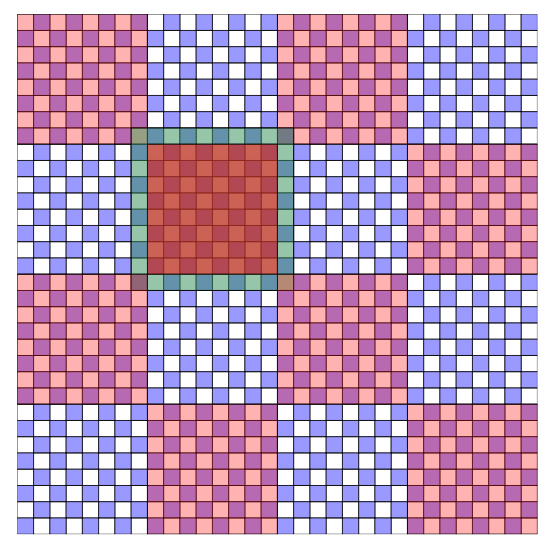
\includegraphics[width=2.5in]{./checkerboard.png}
\caption[]{ Double checkerboard decomposition of a square lattice of edge length L=32 onto 16 processors, each processor is assigned a tile of $8 \times 8$ sites. Taken from \cite{Weigel}}
\label{sample-figure}
\end{center}
\end{figure}
The updating procedure looks as follows \cite{Weigel}:
\begin{enumerate}
\item The $L \times L$ lattice is evenly decomposed into N processors, where $\sqrt{N}$ is an integer and L is divisible by $\sqrt{N}$. 
\item Each processor initialize the spin configuration of their tile.
\item Each processor performs a Metropolis update of each lattice site in their tile in parallel.
\item The threads of each processor are synchronized.
\item Steps 3 to 4 are repeated until the system is thermalized.
\end{enumerate}

\subsection{Data analysis}
With fixed temperature,  we will study  the thermalization time and analyze the performance of the serial code and parallel code with speedup.

\section{Analysis}
With the lattice size L = 1024, we will simulate the system using both serial and parallel code with N = 4, 16, 64, 256 and 1024. Weak scaling can also be measured with fixed load on each processors. We will test our code on JANUS and other platforms that available to us.


% ---- Bibliography ----
%
\begin{thebibliography}{99}
\bibitem{Young}
http://young.physics.ucsc.edu/ising/ising.html
\bibitem{Weigel}
Martin Weigel, J. Comput. Phys. 231, 3064 (2012).
\bibitem{Drexel}
http://www.pages.drexel.edu/~cfa22/msim/node10.html 
\bibitem{Newman}
M. E. J. Newman and G. T. Barkema. Monte Carlo Methods in Statistical Physics. Oxford, 2009.
\end{thebibliography}
\end{document}

